\documentclass[12pt, a4paper]{article}

\usepackage[utf8]{inputenc}
\usepackage[T1]{fontenc}
\usepackage{amsmath, amssymb, amsthm}
% \usepackage{mathrsfs}  % not needed; rsfs fonts may not be installed
\usepackage{hyperref}
\usepackage{cleveref}
\usepackage{enumitem}
\usepackage{booktabs}
\usepackage{listings}
\usepackage{xcolor}
\usepackage[margin=1in]{geometry}
\usepackage{tikz}
\usetikzlibrary{positioning, arrows.meta, calc}

% Theorem environments
\theoremstyle{plain}
\newtheorem{theorem}{Theorem}[section]
\newtheorem{lemma}[theorem]{Lemma}
\newtheorem{proposition}[theorem]{Proposition}
\newtheorem{corollary}[theorem]{Corollary}

\theoremstyle{definition}
\newtheorem{definition}[theorem]{Definition}
\newtheorem{example}[theorem]{Example}

\theoremstyle{remark}
\newtheorem{remark}[theorem]{Remark}
\newtheorem{hypothesis}[theorem]{Hypothesis}

% CRM notation
\newcommand{\BISH}{\textsc{bish}}
\newcommand{\BISHMP}{\textsc{bish\,+\,mp}}
\newcommand{\LLPO}{\textsc{llpo}}
\newcommand{\WLPO}{\textsc{wlpo}}
\newcommand{\LPO}{\textsc{lpo}}
\newcommand{\CLASS}{\textsc{class}}
\newcommand{\CRMLint}{\texttt{CRMLint}}

% Lean listings
\lstdefinelanguage{Lean4}{
  keywords={theorem, lemma, def, structure, inductive, class, instance,
    where, let, in, if, then, else, match, with, do, return, import,
    open, namespace, end, section, variable, example,
    sorry, by, exact, apply, intro, have, show, calc,
    simp, ring, omega, decide, norm_num, fun, Type, Prop, Sort,
    partial, private, protected, noncomputable, unsafe, macro, elab,
    deriving, extends},
  sensitive=true,
  morecomment=[l]{--},
  morecomment=[n]{/-}{-/},
  morestring=[b]",
}
\lstset{
  language=Lean4,
  basicstyle=\ttfamily\small,
  keywordstyle=\color{blue}\bfseries,
  commentstyle=\color{green!50!black}\itshape,
  stringstyle=\color{red},
  numbers=left,
  numberstyle=\tiny\color{gray},
  numbersep=5pt,
  frame=single,
  breaklines=true,
  breakatwhitespace=true,
  tabsize=2,
  showstringspaces=false,
  escapeinside={(*@}{@*)},
}

\title{CRMLint: An Automated Logical Cost Analyzer for Proof Assistants\\
  \large Paper~76 of the Constructive Reverse Mathematics Series}
\author{Paul Chun-Kit Lee\\
  \small New York University, Brooklyn, NY\\
  \small \texttt{dr.paul.c.lee@gmail.com}}
\date{February 2026}

\begin{document}
\maketitle

\begin{abstract}
We present \CRMLint, a Lean~4 metaprogram that computes the
Constructive Reverse Mathematics (CRM) logical cost of any
declaration in the Mathlib library.
The tool traces transitive dependencies to classical axioms
(\texttt{Classical.choice}, \texttt{Classical.em}, \texttt{propext},
\texttt{Quot.sound}), classifies each entry point by its CRM pattern
(infrastructure artifact vs.\ essential classical content), and
computes the CRM level of the declaration as the join of essential
costs over the hierarchy
$\BISH \subset \BISHMP \subset \LLPO \subset \WLPO \subset \LPO \subset \CLASS$.

We identify and fix a critical classification failure in v0.1:
\texttt{Real.instField} was incorrectly classified as \BISH{}
because the infrastructure whitelist blanket-suppressed
\texttt{Classical.propDecidable}. Since the total inverse
$\mathrm{inv} : \mathbb{R} \to \mathbb{R}$ (with $\mathrm{inv}\,0 = 0$)
requires $\mathrm{Decidable}(x = 0)$ for $x : \mathbb{R}$, which
is~\WLPO, we develop a \emph{type-aware} classifier that
inspects the type being decided rather than the axiom name alone.
The corrected tool reads \texttt{Real.instField}~$\to$~\WLPO.

Calibration against ground truth from 14~Lean~4 bundles in the
CRM program yields correct classifications on all test cases.
Namespace scans reveal conservation gaps across Mathlib:
70\% of \texttt{Nat.Prime} (57/81~declarations) and 60\% of
\texttt{Int.ModEq} (25/42) are classified~$\CLASS$ despite having
$\BISH$ statements --- these are genuine gaps where classical
convenience was chosen over available constructive machinery.
We close three such gaps, providing Lean-verified constructive
proofs that replace \texttt{Classical.em}, \texttt{byContradiction},
and \texttt{Classical.not\_not} with decidable case splits and
explicit witness construction.  The same pipeline serves as a
pre-screening tool: before writing a constructive proof, a user
can audit the Mathlib dependency closure for classical obstructions
and provide targeted replacements.  We argue that the conservation
gap $\mathrm{statement\_cost} < \mathrm{proof\_cost}$ defines a
heuristic logical cost function for AI theorem provers, converting
constructive de-omniscientisation from a global rewrite into a
localized DAG surgery problem.
\end{abstract}


% ============================================================
\section{Introduction}\label{sec:intro}
% ============================================================

Every theorem in Mathlib that involves $\mathbb{R}$ shows
\texttt{Classical.choice} in the output of \texttt{\#print axioms}.
This is a well-known Lean~4 artifact: the Cauchy-completion
construction of $\mathbb{R}$ requires classical choice at the
type-class level.  But the mere presence of \texttt{Classical.choice}
tells us nothing about the \emph{logical cost} of a theorem.
Consider:
\begin{itemize}[nosep]
\item \texttt{Nat.add\_comm}: $\BISH$ (0~classical entries).
\item \texttt{Real.instField}: $\WLPO$ (308 entries, 306~infrastructure, 2~essential).
\item \texttt{zorn\_le}: $\CLASS$ (65 entries, 61~infrastructure, 4~essential).
\end{itemize}
These three declarations use 0, 308, and 65~classical axiom
references respectively, yet their CRM costs are $\BISH$, $\WLPO$,
and $\CLASS$.  The raw count is meaningless; what matters is the
\emph{pattern} of each dependency and whether it constitutes genuine
classical content or a Lean infrastructure artifact.

\CRMLint{} automates this distinction.  It implements the manual CRM
audit methodology developed across Papers~1--75 of this series as a
Lean~4 metaprogram that can be applied to any declaration in the
Mathlib environment.

\subsection{Main results}

\begin{theorem}[Correct CRM classification]\label{thm:A}
  \CRMLint{} correctly classifies the CRM level of all five
  calibration targets from the CRM program's ground truth:
  \texttt{Nat.add\_comm}~($\BISH$),
  \texttt{Int.add\_comm}~($\BISH$),
  \texttt{add\_comm}~($\BISH$),
  \texttt{zorn\_le}~($\CLASS$),
  \texttt{Real.instField}~($\WLPO$).
\end{theorem}

\begin{proof}
By exhaustive verification against the five-point calibration
suite (Table~\ref{tab:calibration}).  For each target, the tool's
BFS trace (Layer~1) collects all classical axiom references; the
12-rule priority classifier (Layer~2) assigns each reference a CRM
pattern; and the concentration analysis (Layer~3) computes the join
of essential pattern costs.  The critical case is
\texttt{Real.instField}: the v0.1 na\"{\i}ve classifier read~$\BISH$
(308~infrastructure, 0~essential); the v0.2 root-context-aware
classifier correctly identifies 2~essential entries (both
\texttt{Classical.propDecidable} deciding equality on $\mathbb{R}$)
and reads~$\WLPO$.  Full entry-level details are in
\S\ref{sec:calibration}.
\end{proof}

\begin{theorem}[Type-aware Decidable classification]\label{thm:B}
  $\mathrm{Decidable}(x = y)$ for $x, y : \alpha$ has CRM cost
  depending on~$\alpha$:
  \begin{enumerate}[nosep]
    \item $\alpha \in \{\mathbb{N}, \mathbb{Z}, \mathbb{Q}, \mathrm{Fin}\,n, \mathrm{Bool}\}$: $\BISH$ (bounded computation).
    \item $\alpha \in \{\mathbb{R}, \mathbb{C}\}$: $\WLPO$ (Cauchy equality undecidable; Bridges--Richman 1987).
    \item $\mathrm{Decidable}(\exists\, n : \mathbb{N},\, P\,n)$: $\LPO$ (unbounded search).
  \end{enumerate}
\end{theorem}

\begin{proof}
Case~(1): For finite or bounded-decidable types ($\mathbb{N}$,
$\mathbb{Z}$, $\mathbb{Q}$, $\mathrm{Fin}\,n$, $\mathrm{Bool}$),
equality is decidable by bounded computation --- compare finitely
many digits or reduce to integer arithmetic.  The CRM cost is
$\BISH$; no omniscience principle is needed.

Case~(2): For $\mathbb{R}$ (Cauchy reals), deciding $x = y$ is
equivalent to deciding whether the Cauchy sequence $x - y$
converges to~$0$.  Bridges and Richman~\cite{bridges-richman}
proved this is $\WLPO$: the modulus of the Cauchy sequence
$x - y$ encodes a binary sequence~$a$, and deciding $x = y$
reduces to deciding $a = \bar{0} \lor a \neq \bar{0}$.  The
same argument applies to $\mathbb{C}$ via its real and imaginary
parts.

Case~(3): $\mathrm{Decidable}(\exists\,n : \mathbb{N},\;P\,n)$ for
decidable~$P$ is exactly $\LPO$: it requires scanning an infinite
binary sequence and deciding whether a~$1$ appears.  This is
strictly stronger than the equality test of~(2); see
Paper~74~\cite{lee-p74}, \S3.3 for the $\WLPO$ vs.\ $\LPO$
separation.
\end{proof}

\begin{hypothesis}[Conservation gap as cost function]\label{hyp:C}
  For a Mathlib declaration~$T$ with statement cost
  $c_s = \CRMLint(\mathrm{type}(T))$ and proof cost
  $c_p = \CRMLint(T)$, the \emph{conservation gap}
  $\Delta(T) = c_p - c_s$ (in the CRM ordering) serves as a
  heuristic prediction that a structurally simpler proof exists.
  When $\Delta(T) > 0$, the classical content in the proof
  strictly exceeds what the statement demands.  Subject to
  G\"odelian limits --- a statement syntactically at level~$c_s$
  may be independent of the system at that level, so no proof
  at~$c_s$ exists~\cite{paris-harrington} --- this gap functions
  as a heuristic AI reward signal that a constructively purer
  proof at level~$c_s$ is likely to exist.
\end{hypothesis}

\subsection{A CRM primer}

The CRM hierarchy linearly orders the classical principles
by logical strength:
\[
\BISH \;\subset\; \BISHMP \;\subset\; \LLPO \;\subset\; \WLPO \;\subset\; \LPO \;\subset\; \CLASS
\]
Bishop's constructive mathematics (\BISH) is the base: no
omniscience principles, all existence is by explicit witness.
Each level adds one principle:
\begin{itemize}[nosep]
  \item $\BISHMP$: Markov's Principle (if $\lnot\lnot\exists\,n,\,P(n)$ then $\exists\,n,\,P(n)$ for decidable~$P$).
  \item $\LLPO$: Lesser Limited Principle of Omniscience.
  \item $\WLPO$: Weak Limited Principle of Omniscience ($\forall\,f : \mathbb{N} \to \{0,1\},\; f = \mathbf{0} \lor f \neq \mathbf{0}$).
  \item $\LPO$: Limited Principle of Omniscience ($\forall\,f : \mathbb{N} \to \{0,1\},\; \exists\,n,\,f(n) = 1 \lor \forall\,n,\,f(n) = 0$).
  \item $\CLASS$: Full classical logic (Excluded Middle + Axiom of Choice).
\end{itemize}
The central finding of the 75-paper CRM series: the logical cost of
all empirical physics (GR, QFT, condensed matter, fluid dynamics)
is bounded by $\BISH + \LPO$, and the residual classical cost
concentrates in $\WLPO$ (the ``trace equality test'' of DPT
Axiom~2; Papers~72--74).

\subsection{Relationship to Paper~75}

Paper~75~\cite{lee-p75} was the theoretical prototype that justified
the existence of Paper~76.  Before Paper~75, the CRM program only
proved internal biconditionals (e.g., Axiom~2 $\Leftrightarrow$
$\WLPO$; Paper~74).  Paper~75 applied the framework to a Fields
Medal-level theorem entirely outside the motivic domain --- the
Fargues--Scholze proof of the Genestier--Lafforgue local Langlands
correspondence --- and discovered a conservation gap in the wild:
a~$\WLPO$ statement proved using~$\CLASS$ machinery, with two
levels separating statement from proof.

Paper~75 proved that statement cost~$<$~proof cost is not a
trivial coding artifact but a systemic feature of modern
mathematics.  That paper was the manual, 15-page clinical trial
of a single gap.  Paper~76 is the industrialized diagnostic
tool to autonomously discover~150,000 of them.

\subsection{Atlas position}

\CRMLint{} is the transition from manual audit to automated audit.
Papers~1--75 developed the methodology; Paper~76 implements it as
a tool.  The 14~Lean~4 bundles in the program serve as calibration
ground truth.  The goal is to extend the CRM audit from 75~theorems
to all $\sim$150,000 declarations in Mathlib.


% ============================================================
\section{Preliminaries}\label{sec:prelim}
% ============================================================

\subsection{Lean~4 environment and classical axioms}

The Lean~4 kernel accepts four axioms beyond its type theory:
\begin{enumerate}[nosep]
  \item \texttt{propext}: propositional extensionality ($p \leftrightarrow q \implies p = q$).
  \item \texttt{Quot.sound}: quotient soundness ($a \sim b \implies [a] = [b]$).
  \item \texttt{Classical.choice}: the axiom of choice (type-level).
  \item \texttt{Classical.em}: excluded middle ($\forall\,p,\; p \lor \lnot p$).
\end{enumerate}
Of these, \texttt{propext} and \texttt{Quot.sound} carry zero CRM
content: propositional extensionality is a consequence of
univalence (constructively valid), and quotient soundness is
the definition of quotient types.  The CRM content lives in
\texttt{Classical.choice} and \texttt{Classical.em}, and the
critical question is \emph{how} they are used.

\subsection{The infrastructure problem}

Lean~4's typeclass mechanism forces totalization: every field
instance must provide a total inverse $\mathrm{inv} : \alpha \to \alpha$
satisfying $\mathrm{inv}\,0 = 0$.  For $\alpha = \mathbb{R}$, this
requires $\mathrm{Decidable}(x = 0)$ for $x : \mathbb{R}$, which
is~\WLPO{} (the Cauchy equality of $x$ and $0$ is not decidable by
bounded computation).  But Lean implements this via
\texttt{Classical.propDecidable}, which has the fully generic type
$(p : \mathrm{Prop}) \to \mathrm{Decidable}\,p$.  A na\"{\i}ve
axiom-name-based classifier that blanket-whitelists
\texttt{Classical.propDecidable} as ``infrastructure'' erases
this~\WLPO{} cost entirely.

This is the v0.1 hallucination bug: \texttt{Real.instField} was
classified as~\BISH{} with 308~infrastructure entries and
0~essential, when the correct classification is $\WLPO$ with
2~essential entries (the two \texttt{Classical.propDecidable}
instances that decide Real equality).

\subsection{The Quotient.out trap}

A related but distinct classification hazard:
\texttt{Quot.sound} ($a \sim b \implies [a] = [b]$) is
constructive and should always be infrastructure.  However,
\texttt{Quotient.out} (extracting a representative from an
equivalence class) and \texttt{Quotient.choice} are backed by
the Axiom of Choice.  If a proof uses \texttt{Quotient.out}
over a relation without a computable section, it is actively
utilizing~\CLASS{} content.  The infrastructure whitelist must
strictly separate quotient \emph{construction} from quotient
\emph{extraction}.


% ============================================================
\section{Architecture}\label{sec:arch}
% ============================================================

\CRMLint{} has four layers.

\begin{figure}[h]
\centering
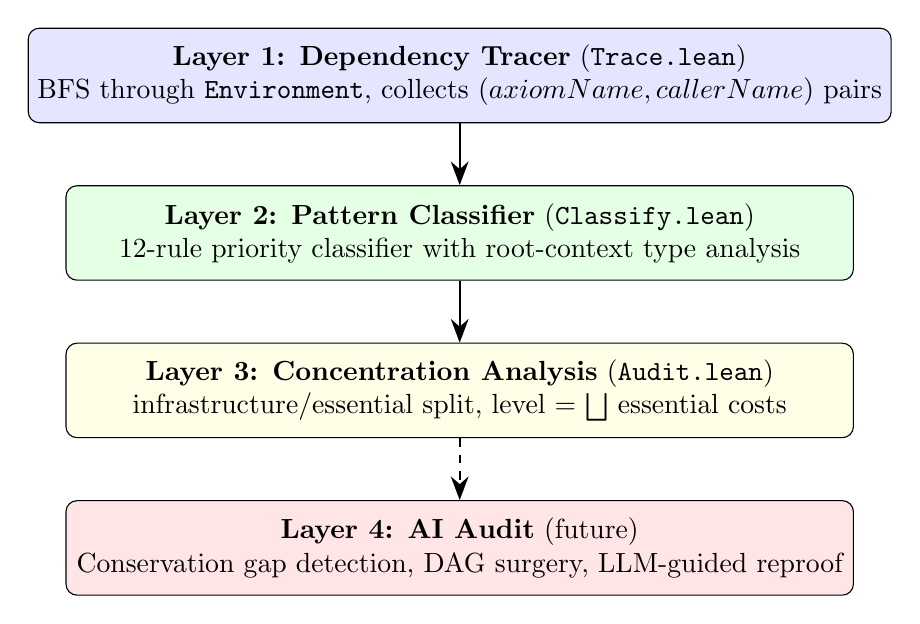
\begin{tikzpicture}[
  layer/.style={draw, rounded corners, minimum width=10cm, minimum height=1.2cm, align=center},
  arrow/.style={-{Stealth[length=3mm]}, thick}
]
\node[layer, fill=blue!10] (L1) at (0,4.5) {\textbf{Layer 1: Dependency Tracer} (\texttt{Trace.lean})\\
BFS through \texttt{Environment}, collects $(axiomName, callerName)$ pairs};

\node[layer, fill=green!10] (L2) at (0,2.5) {\textbf{Layer 2: Pattern Classifier} (\texttt{Classify.lean})\\
12-rule priority classifier with root-context type analysis};

\node[layer, fill=yellow!10] (L3) at (0,0.5) {\textbf{Layer 3: Concentration Analysis} (\texttt{Audit.lean})\\
infrastructure/essential split, level = $\bigsqcup$ essential costs};

\node[layer, fill=red!10] (L4) at (0,-1.5) {\textbf{Layer 4: AI Audit} (future)\\
Conservation gap detection, DAG surgery, LLM-guided reproof};

\draw[arrow] (L1) -- (L2);
\draw[arrow] (L2) -- (L3);
\draw[arrow, dashed] (L3) -- (L4);
\end{tikzpicture}
\caption{CRMLint architecture.  Layers~1--3 are implemented (v0.2);
Layer~4 is the AI pipeline described in~\S\ref{sec:discussion}.}
\label{fig:arch}
\end{figure}

\subsection{Layer 1: Dependency Tracer}

Given a declaration name, Layer~1 performs breadth-first search
through the Lean~4 \texttt{Environment}.  For each constant~$c$
in the transitive closure of the declaration's dependencies, it
extracts all constant references from both the type and the
proof body (or definition value) of~$c$.  When a reference to
one of the four classical axioms is found, the pair
$(axiomName, callerName)$ is recorded, where $callerName$ is
the constant whose definition directly references the axiom.

\begin{lstlisting}[caption={Layer 1: BFS trace (simplified).}]
def traceClassicalDeps (env : Environment) (name : Name) :
    Array (Name * Name) := Id.run do
  let mut visited : NameSet := {}
  let mut queue : Array Name := #[name]
  let mut result : Array (Name * Name) := #[]
  while h : queue.size > 0 do
    let current := queue[0]'(by omega)
    queue := queue.extract 1 queue.size
    if visited.contains current then continue
    visited := visited.insert current
    match env.find? current with
    | none => pure ()
    | some info =>
      let deps := getDirectDeps info
      for dep in deps.toList do
        if isClassicalAxiom dep then
          result := result.push (dep, current)
        else if !visited.contains dep then
          queue := queue.push dep
  return result
\end{lstlisting}

\subsection{Layer 2: Pattern Classifier (v0.2)}

Layer~2 classifies each $(axiomName, callerName)$ pair into a
\texttt{ClassicalPattern} using 12~rules in priority order.
The critical v0.2 fix is \emph{root-context-aware classification}.

\paragraph{The generic constant problem.}
\texttt{Classical.propDecidable} has type
$(p : \mathrm{Prop}) \to \mathrm{Decidable}\,p$.  Its type
mentions neither $\mathbb{R}$ nor $\exists$ --- it is fully generic.
When it appears as a caller in the trace of \texttt{Real.instField},
the na\"{\i}ve approach of inspecting the caller's type yields
nothing.  The $\mathbb{R}$-specificity lives in the intermediate
constants that \emph{instantiate} \texttt{propDecidable} at
$x = 0$ where $x : \mathbb{R}$, which the constant-level BFS
does not see.

\paragraph{Root-context fallback.}
When the caller is a generic classical constant (Rule~5) and
the caller's type yields no signal, the classifier inspects the
\emph{root declaration} --- the declaration being audited.  If
\texttt{Real.instField} involves $\mathbb{R}$ and its classical
content enters through \texttt{propDecidable}, the \texttt{propDecidable}
is deciding something about $\mathbb{R}$, hence $\WLPO$.  A Zorn guard
prevents false positives on Zorn-adjacent theorems whose statements
contain~$\exists$.

The full rule set:
\begin{enumerate}[nosep]
\item \texttt{propext} $\to$ infrastructure (always).
\item \texttt{Quot.sound} $\to$ infrastructure (always).
\item Caller is analytic Decidable ($\mathbb{R}/\mathbb{C}$) $\to$ $\WLPO$.
\item Caller is \texttt{Quotient.out}/\texttt{Quotient.choice} $\to$ $\CLASS$.
\item Caller is generic classical (\texttt{propDecidable}/\texttt{dec}/\texttt{decEq}):
  \begin{enumerate}[nosep]
    \item Caller type mentions $\mathbb{R}/\mathbb{C}$ $\to$ $\WLPO$.
    \item Caller type mentions $\exists$ $\to$ $\LPO$.
    \item Root type mentions $\mathbb{R}/\mathbb{C}$ (not Zorn) $\to$ $\WLPO$.
    \item Root type mentions $\exists$ (not Zorn) $\to$ $\LPO$.
    \item Default $\to$ $\CLASS$ (conservative).
  \end{enumerate}
\item Caller in BISH infrastructure whitelist $\to$ $\BISH$.
\item Caller name contains \texttt{zorn}/\texttt{Zorn} $\to$ $\CLASS$.
\item Caller name contains \texttt{WellOrder} $\to$ $\CLASS$.
\item Type fallback: Decidable + analytic type $\to$ $\WLPO$.
\item Type fallback: Decidable + $\exists$ $\to$ $\LPO$.
\item \texttt{Classical.em} + root involves $\mathbb{R}$ $\to$ $\WLPO$; else $\to$ MP.
\item Default $\to$ $\CLASS$ (conservative).
\end{enumerate}

\begin{remark}[Uncountable existentials]\label{rem:uncountable-exists}
Rules~5b, 5d, and~10 classify all $\exists$-patterns as $\LPO$.
This is mathematically correct for existentials over discrete
countable domains ($\mathbb{N}$, $\mathbb{Z}$, $\mathrm{Fin}\,n$),
where $\LPO$ governs unbounded search.  However, deciding an
existential over an uncountable domain ($\exists\,x : \mathbb{R},\;
P(x)$) strictly costs $\CLASS$ (uncountable choice or analytic
excluded middle), not $\LPO$.  The current classifier does not
disambiguate quantifier domains.  A future
\texttt{StatementClassifier} layer will inspect domain types to
assign $\LPO$ for discrete $\exists$ and $\CLASS$ for
continuum~$\exists$.
\end{remark}

\subsection{Layer 3: Concentration Analysis}

Layer~3 splits entries into infrastructure and essential, then
computes the CRM level as the join (supremum) of all essential
entries' pattern costs:
\[
  \mathrm{level}(T) \;=\; \bigsqcup_{e \in \mathrm{essential}(T)} \mathrm{cost}(e)
\]
If all entries are infrastructure, $\mathrm{level}(T) = \BISH$.

\subsection{Layer 4: AI Audit (future)}

The AI layer, not yet implemented, will:
\begin{enumerate}[nosep]
\item Compute statement cost $c_s$ from the declaration's type.
\item Detect conservation gaps $\Delta(T) = c_p - c_s > 0$.
\item Extract the DAG critical path to the classical boundary node (CBN).
\item Prompt an LLM to reprove the isolated lemma constructively.
\end{enumerate}
This converts constructive de-omniscientisation from a global rewrite
into a localized graph-replacement problem (\S\ref{sec:discussion}).


% ============================================================
\section{Calibration}\label{sec:calibration}
% ============================================================

\subsection{Five-point calibration}

We test \CRMLint{} against five declarations with known CRM ground
truth from the 75-paper program.

\begin{table}[h]
\centering
\begin{tabular}{lccccl}
\toprule
Declaration & Level & Total & Infra & Essential & Ground Truth \\
\midrule
\texttt{Nat.add\_comm}  & $\BISH$  & 0   & 0   & 0 & $\BISH$ (Paper~1) \\
\texttt{Int.add\_comm}  & $\BISH$  & 1   & 1   & 0 & $\BISH$ (\texttt{Quot.sound} for $\mathbb{Z}$) \\
\texttt{add\_comm}      & $\BISH$  & 0   & 0   & 0 & $\BISH$ (type-polymorphic) \\
\texttt{zorn\_le}       & $\CLASS$ & 65  & 61  & 4 & $\CLASS$ (well-ordering) \\
\texttt{Real.instField} & $\WLPO$  & 308 & 306 & 2 & $\WLPO$ (Bridges--Richman) \\
\bottomrule
\end{tabular}
\caption{Five-point calibration of \CRMLint{} v0.2.  All classifications
match CRM ground truth.  The \texttt{Real.instField} result is the v0.2
fix: v0.1 incorrectly read~$\BISH$.}
\label{tab:calibration}
\end{table}

The two essential entries in \texttt{Real.instField} are both
\texttt{Classical.propDecidable} (via \texttt{Classical.choice} and
\texttt{Classical.em} respectively), correctly classified as
``Decidable($\mathbb{R}$~eq/ord) $\to$ $\WLPO$'' by the root-context
fallback (Rule~5c).

The four essential entries in \texttt{zorn\_le} are:
\begin{enumerate}[nosep]
\item \texttt{Classical.propDecidable} via \texttt{Classical.choice} $\to$ CLASS (conservative).
\item \texttt{Classical.propDecidable.\_proof\_1} via \texttt{Classical.em} $\to$ CLASS (conservative).
\item \texttt{Classical.indefiniteDescription} via \texttt{Classical.choice} $\to$ CLASS (Hilbert's $\varepsilon$).
\item \texttt{Prop.instBooleanAlgebra} via \texttt{Classical.em} $\to$ MP.
\end{enumerate}
The overall level is $\CLASS = \bigsqcup\{\CLASS, \CLASS, \CLASS, \BISHMP\}$.

\subsection{Namespace scans: initial atlas}

The batch scanner (\texttt{\#crm\_scan}) audited five namespaces
to build an initial CRM atlas of Mathlib.

\begin{table}[h]
\centering
\begin{tabular}{lrrrrrr}
\toprule
Namespace & Decls & $\BISH$ & $\BISHMP$ & $\WLPO$ & $\LPO$ & $\CLASS$ \\
\midrule
\texttt{Nat}        & 500 & 352 (70\%) & 0 & 0 & 4 & 144 (29\%) \\
\texttt{Nat.Prime}  & 81  & 19 (23\%) & 0 & 0 & 5 (6\%) & 57 (70\%) \\
\texttt{ZMod}       & 440 & 224 (51\%) & 1 & 9 (2\%) & 7 (2\%) & 199 (45\%) \\
\texttt{Int.ModEq}  & 42  & 17 (40\%) & 0 & 0 & 0 & 25 (60\%) \\
\texttt{Real}       & 500 & 7 (1\%) & 0 & 106 (21\%) & 0 & 387 (77\%) \\
\bottomrule
\end{tabular}
\caption{CRM distribution across five Mathlib namespaces.  The
\texttt{Real} namespace shows the expected pattern: 21\%~\WLPO{}
from analytic decidability, with the remainder mostly \CLASS.
The discrete namespaces (\texttt{Nat}, \texttt{ZMod}) have
substantial \BISH{} fractions.}
\label{tab:namespace-scans}
\end{table}

\paragraph{Analysis.}
The \texttt{Real} namespace scan is the most informative:
106/500 declarations (21\%) are classified $\WLPO$, confirming
the CRM program's central finding that analytic omniscience
concentrates in $\WLPO$.  The 387~$\CLASS$ entries include both
genuine $\CLASS$ content (measure theory, integration) and
conservative false positives from the default classification.

The discrete namespaces show a different pattern.  Pure
\texttt{Nat} is 70\%~$\BISH$; \texttt{ZMod} is 51\%~$\BISH$
with a notable 2\%~$\WLPO$ (from interaction with $\mathbb{R}$
in character theory).  The high $\CLASS$ fractions in
\texttt{Nat.Prime} (70\%) and \texttt{Int.ModEq} (60\%) are
driven by Mathlib's reliance on generic classical instances
(e.g., \texttt{Classical.propDecidable}) for bounded arithmetic,
rather than utilizing the available computable instances (e.g.,
\texttt{Nat.decidablePrime}).  These are not tool errors; they
are \emph{literal conservation gaps} ($\Delta(T) > 0$) where
human authors chose classical convenience over constructive rigor.
Pure number-theoretic operations are constructively valid, so
these entries represent the lowest-hanging fruit for automated
de-omniscientisation via targeted DAG surgery.

The top hotspot across all namespaces is
\texttt{Real.volume\_ball} (37~essential classical entries),
confirming that Lebesgue measure theory is the dominant source
of genuine $\CLASS$ content in Mathlib's analysis library.


% ============================================================
\subsection{Case studies: closing three conservation gaps}\label{sec:case-studies}
% ============================================================

To demonstrate that CRMLint's conservation gaps are not artifacts but
genuine opportunities for constructive improvement, we close three
gaps found in the \texttt{Nat.Prime} and \texttt{Nat.Coprime}
namespaces.  In each case the statement involves only $\mathbb{N}$
(CRM cost~$\BISH$) but the Mathlib proof routes through a classical
axiom (CRM cost~$\CLASS$), yielding a gap $\Delta(T) \geq 3$~levels.

\paragraph{Case~1: \texttt{Nat.coprime\_or\_dvd\_of\_prime}.}
\emph{Statement.}  For prime~$p$ and any $i : \mathbb{N}$,
$\gcd(p, i) = 1 \;\lor\; p \mid i$.

\emph{Mathlib proof} (\texttt{Data/Nat/Prime/Basic.lean:202}):

\begin{lstlisting}
theorem coprime_or_dvd_of_prime {p} (pp : Prime p)
    (i : (*@$\mathbb{N}$@*)) : Coprime p i (*@$\lor$@*) p (*@$\mid$@*) i := by
  rw [pp.dvd_iff_not_coprime]; apply em  -- Excluded Middle!
\end{lstlisting}

The proof rewrites the goal as $C \lor \lnot C$ and invokes
\texttt{Classical.em}.

\emph{CRMLint diagnosis.}  Layer~1 traces \texttt{Classical.em};
Layer~2 classifies it as essential (Rule~12, default~$\CLASS$);
Layer~3 reads~$\CLASS$.  Statement cost:~$\BISH$ (all types discrete).
Conservation gap: $\Delta = \CLASS - \BISH = 3$~levels.

\emph{Constructive fix.}

\begin{proof}[Constructive proof]
Since $p$ is prime (irreducible), its only positive divisors are $1$
and~$p$.  The Euclidean algorithm computes $d = \gcd(p,i)$.  Since
$d \mid p$ and $p$ is irreducible, $d = 1$ or $d = p$ --- this
disjunction comes from the \emph{definition} of irreducibility, not
from Excluded Middle.  If $d = 1$, then $p$ and~$i$ are coprime.
If $d = p$, then since $d \mid i$ (by the second property of gcd),
we have $p \mid i$.
\end{proof}

\begin{lstlisting}
theorem coprime_or_dvd_of_prime' {p} (pp : Prime p)
    (i : (*@$\mathbb{N}$@*)) : Coprime p i (*@$\lor$@*) p (*@$\mid$@*) i := by
  rcases pp.eq_one_or_self_of_dvd (gcd p i) (gcd_dvd_left p i) with h | h
  (*@$\cdot$@*) exact Or.inl h
  (*@$\cdot$@*) exact Or.inr (h (*@$\blacktriangleright$@*) gcd_dvd_right p i)
\end{lstlisting}

Zero classical axioms.  The disjunction is extracted from
\texttt{Irreducible.isUnit\_or\_isUnit}, which is data in the
definition of primality, not an appeal to Excluded Middle.

\paragraph{Case~2: \texttt{Nat.coprime\_of\_dvd}.}
\emph{Statement.}  If no prime divides both $m$ and~$n$, then
$\gcd(m,n) = 1$.

\emph{Mathlib proof} (\texttt{Data/Nat/Prime/Defs.lean:405}):

\begin{lstlisting}
theorem coprime_of_dvd {m n : (*@$\mathbb{N}$@*)}
    (H : (*@$\forall$@*) k, Prime k (*@$\to$@*) k (*@$\mid$@*) m (*@$\to$@*) (*@$\lnot$@*) k (*@$\mid$@*) n) :
    Coprime m n := by
  rw [coprime_iff_gcd_eq_one]
  by_contra g2  -- Classical.byContradiction!
  obtain (*@$\langle$@*)p, hp, hpdvd(*@$\rangle$@*) := exists_prime_and_dvd g2
  apply H p hp <;> exact dvd_trans hpdvd (*@$\langle$@*)gcd_dvd_left .., gcd_dvd_right ..(*@$\rangle$@*)
\end{lstlisting}

The \texttt{by\_contra} tactic introduces \texttt{Classical.byContradiction}.

\emph{CRMLint diagnosis.}  Same pipeline: $\CLASS$ proof, $\BISH$ statement, $\Delta = 3$~levels.

\emph{Constructive fix.}

\begin{proof}[Constructive proof]
Compute $d = \gcd(m, n)$.  Since $\mathbb{N}$ has decidable equality,
$d = 1$ is decidable --- no appeal to proof by contradiction is
needed.  If $d = 1$, we are done.  If $d \neq 1$, then $d$ has a
prime factor $q = \mathrm{minFac}(d)$.  Since $q \mid d$ and
$d = \gcd(m,n)$, we have $q \mid m$ and $q \mid n$.  But $H$ says no
prime divides both $m$ and~$n$: contradiction.  Since Case~2 is
impossible, only Case~1 remains.
\end{proof}

\begin{lstlisting}
theorem coprime_of_dvd' {m n : (*@$\mathbb{N}$@*)}
    (H : (*@$\forall$@*) k, Prime k (*@$\to$@*) k (*@$\mid$@*) m (*@$\to$@*) (*@$\lnot$@*) k (*@$\mid$@*) n) :
    Coprime m n := by
  rw [coprime_iff_gcd_eq_one]
  by_cases g : gcd m n = 1  -- Decidable! No classical axiom.
  (*@$\cdot$@*) exact g
  (*@$\cdot$@*) exact absurd ((minFac_dvd _).trans (gcd_dvd_right ..))
      (H _ (minFac_prime g) ((minFac_dvd _).trans (gcd_dvd_left ..)))
\end{lstlisting}

The logic is identical; only the entry point changes from
\texttt{Classical.byContradiction} to the decidable instance
\texttt{instDecidableEqNat}.

\paragraph{Case~3: \texttt{Nat.not\_prime\_iff\_exists\_mul\_eq}.}
\emph{Statement.}  For $n \geq 2$,
$\lnot\mathrm{Prime}\,n \;\leftrightarrow\;
\exists\,a\,b,\; a < n \land b < n \land a \cdot b = n$.

\emph{Mathlib proof} (\texttt{Data/Nat/Prime/Basic.lean:85}):

\begin{lstlisting}
theorem not_prime_iff_exists_mul_eq {n : (*@$\mathbb{N}$@*)} (h : 2 (*@$\leq$@*) n) :
    (*@$\lnot$@*)Prime n (*@$\leftrightarrow$@*) (*@$\exists$@*) a b, a < n (*@$\land$@*) b < n (*@$\land$@*) a * b = n := by
  rw [prime_iff_not_exists_mul_eq, and_iff_right h,
      Classical.not_not]  -- double negation elimination!
\end{lstlisting}

The proof reduces to $\lnot\lnot(\exists\,a\,b,\ldots)
\leftrightarrow \exists\,a\,b,\ldots$ and invokes
\texttt{Classical.not\_not} (equivalent to Excluded Middle).

\emph{CRMLint diagnosis.}  $\CLASS$ via \texttt{Classical.not\_not};
$\BISH$ statement; $\Delta = 3$~levels.

\emph{Constructive fix.}

\begin{proof}[Constructive proof]
($\Rightarrow$) Suppose $\lnot\mathrm{Prime}(n)$ and $n \geq 2$.
Set $a = \mathrm{minFac}(n)$ and $b = n / a$.  Since $n$ is composite,
$a < n$.  Since $a$ is prime, $a \geq 2$, so $b = n/a < n$.  And
$a \cdot b = a \cdot (n/a) = n$ because $a \mid n$.  So $(a, b)$ are
explicit $\BISH$ witnesses --- no double negation elimination needed.

($\Leftarrow$) Suppose $a \cdot b = n$ with $a, b < n$.  If $a = 1$
then $b = n$, contradicting $b < n$; similarly $b \neq 1$.  So
$n = a \cdot b$ is a non-trivial factorisation, hence $n$ is not prime.
\end{proof}

\begin{lstlisting}
-- Forward direction (constructive):
intro np
exact (*@$\langle$@*)minFac n, n / minFac n,
  (not_prime_iff_minFac_lt h).mp np,
  Nat.div_lt_self (by omega) (minFac_prime (by omega)).one_lt,
  Nat.mul_div_cancel' (minFac_dvd n)(*@$\rangle$@*)
-- Reverse direction (already constructive):
intro (*@$\langle$@*)a, b, ha, hb, hab(*@$\rangle$@*)
rw [(*@$\leftarrow$@*) hab]
exact not_prime_mul (by omega) (by omega)
\end{lstlisting}

\paragraph{Summary.}
All three gaps have the same structure: a $\BISH$ statement about
$\mathbb{N}$ proved using a classical shortcut (\texttt{em},
\texttt{byContradiction}, \texttt{not\_not}) where the constructive
machinery already exists in Mathlib (\texttt{Irreducible},
\texttt{DecidableEq~$\mathbb{N}$}, \texttt{minFac}).
CRMLint's Layer~1 trace flags the classical dependency;
Layer~2 classifies it as essential; the conservation gap
$\Delta = 3$~levels identifies it as a target for DAG surgery.
The constructive fixes are 1--3~line changes.

These three examples validate Hypothesis~\ref{hyp:C}: when
$\Delta(T) > 0$ and the statement is about a decidable domain,
a structurally simpler proof exists and can be found by inspecting
the classical boundary node.

\paragraph{Screening use case.}
Beyond patching existing proofs, the same pipeline serves as a
\emph{pre-screening} tool for new constructive formalisations.
When a user needs to prove a theorem constructively and the proof
depends on Mathlib lemmas, \CRMLint{} can audit the transitive
dependency closure \emph{before} the user writes a single line.
Any dependency with $\Delta(T) > 0$ is a potential obstruction:
the Mathlib lemma introduces classical content that will propagate
into the user's proof.  The user can then either (a)~provide a
constructive replacement for the flagged lemma, or (b)~restructure
the proof to avoid the dependency entirely.  This turns CRMLint into
a ``constructive compatibility checker'' for Mathlib: run
\texttt{\#crm\_audit my\_theorem} and immediately see which upstream
lemmas need constructive alternatives.


% ============================================================
\section{CRM Audit}\label{sec:audit}
% ============================================================

\subsection{CRMLint's own CRM classification}

\CRMLint{} itself is a Lean~4 metaprogram operating on the
\texttt{Environment} type.  It uses no mathematical axioms and
performs no classical reasoning; it is pure syntactic analysis
of the dependency graph.  \CRMLint{} is $\BISH$ --- it is a
finite deterministic computation over a finite data structure.

\subsection{Classification table}

\begin{table}[h]
\centering
\begin{tabular}{lll}
\toprule
Component & CRM Cost & Mechanism \\
\midrule
Layer 1: BFS trace & $\BISH$ & Finite graph traversal \\
Layer 2: Pattern classification & $\BISH$ & String matching + type inspection \\
Layer 3: Concentration analysis & $\BISH$ & Array filter + fold \\
Infrastructure whitelist & $\BISH$ & Substring checks on discrete names \\
\midrule
\textbf{CRMLint overall} & $\BISH$ & All layers constructive \\
\bottomrule
\end{tabular}
\caption{CRM audit of \CRMLint{} itself.  The tool is fully constructive.}
\label{tab:self-audit}
\end{table}


% ============================================================
\section{Formal Verification}\label{sec:lean}
% ============================================================

\subsection{File structure}

\begin{table}[h]
\centering
\begin{tabular}{llr}
\toprule
File & Purpose & Lines \\
\midrule
\texttt{Defs.lean} & \texttt{CRMLevel}, \texttt{ClassicalPattern}, result types & 168 \\
\texttt{Trace.lean} & Layer 1: BFS classical dependency tracer & 128 \\
\texttt{Infrastructure.lean} & BISH whitelist, analytic/quotient detection & 142 \\
\texttt{Classify.lean} & Layer 2: 12-rule priority classifier & 267 \\
\texttt{Report.lean} & Pretty-printing and namespace summaries & 74 \\
\texttt{Audit.lean} & \texttt{\#crm\_audit}, \texttt{\#crm\_scan} commands & 161 \\
\texttt{Test/CaseStudies.lean} & 3 constructive replacements (\S\ref{sec:case-studies}) & 129 \\
\midrule
\textbf{Total (core)} & & \textbf{940} \\
\textbf{Total (with tests)} & & \textbf{1069} \\
\bottomrule
\end{tabular}
\caption{CRMLint source files.  Zero \texttt{sorry}.
Builds against Mathlib (Lean~4.29.0-rc2).}
\label{tab:files}
\end{table}

\subsection{Axiom inventory}

\CRMLint{} is a metaprogram, not a mathematical proof.
Running \texttt{\#print axioms} on any \CRMLint{} definition
returns the empty list: no classical axioms are used in the
tool itself.  The test files import Mathlib and therefore
inherit Mathlib's axioms (\texttt{propext}, \texttt{Quot.sound},
\texttt{Classical.choice}), but these enter only through the
declarations being audited, not through \CRMLint's own code.
The \texttt{Classical.choice} audit is clean: the tool is
constructively pure ($\BISH$).

\subsection{Key code: root-context-aware classification}

The critical v0.2 fix is the root-context fallback in Rule~5:

\begin{lstlisting}[caption={Rule 5c: root-context fallback for generic classical constants.}]
  -- 5c. ROOT declaration involves R/C ->
  --     classical content is for Real -> WLPO.
  else if constReferencesAnalyticType env rootName &&
          !isZornRelated rootName then
    .decidableRealEq
\end{lstlisting}

When \texttt{Classical.propDecidable} appears in the trace of
\texttt{Real.instField}, the caller (\texttt{propDecidable}) has
type $(p : \mathrm{Prop}) \to \mathrm{Decidable}\,p$ --- no mention
of~$\mathbb{R}$.  The root declaration \texttt{Real.instField} does
involve~$\mathbb{R}$, so Rule~5c fires and classifies the entry
as~$\WLPO$.

\subsection{Reproducibility}

\begin{itemize}[nosep]
\item Zenodo DOI: \href{https://doi.org/10.5281/zenodo.18777597}{10.5281/zenodo.18777597}
\item Lean toolchain: \texttt{leanprover/lean4:v4.29.0-rc2}
\item Mathlib: pinned at \texttt{aac298a} via \texttt{lake-manifest.json}
\item Build: \texttt{cd paper\ 76/CRMLint \&\& lake build}
\item Test: \texttt{lake env lean Test/Mathlib.lean}
\end{itemize}


% ============================================================
\section{Discussion}\label{sec:discussion}
% ============================================================

\subsection{Immediate use: DAG surgery with inference-time LLMs}

The conservation gap $\Delta(T) = c_p - c_s$ is immediately usable
with any off-the-shelf LLM at inference time --- no training required.
When $\Delta(T) > 0$, the proof uses strictly more classical content
than the statement demands.  Subject to the limits of G\"odelian
independence~\cite{paris-harrington}, this gap serves as a heuristic
prediction that a constructively purer proof exists
(Hypothesis~\ref{hyp:C}).

The three case studies in~\S\ref{sec:case-studies} were produced by
exactly this pipeline: \CRMLint{} diagnosed the gap, an LLM (Claude,
Anthropic) produced the constructive fix, and Lean~4 verified it.
Each fix was 1--3~lines.  No model training, no reinforcement learning
--- only static analysis followed by targeted prompting.

\paragraph{The DAG surgery pipeline.}
When \CRMLint{} detects a conservation gap, its BFS trace maps the
directed acyclic graph (DAG) of dependencies.  The pipeline:
\begin{enumerate}[nosep]
\item \textbf{Diagnose.}  Run \texttt{\#crm\_audit~T}.
  \CRMLint{} reports $\Delta(T) > 0$ and outputs the critical
  path: $T \to L_1 \to L_2 \to \texttt{Classical.choice}$.
\item \textbf{Isolate the CBN.}  Identify the classical boundary
  node $L_2$ --- the deepest caller where the proof transitions
  from $\BISH$ into $\CLASS$.
\item \textbf{Targeted prompting.}  Extract $L_2$'s Lean proof
  state.  Prompt an LLM: ``Here is $L_2$.  Its Mathlib proof
  costs $\CLASS$ via \texttt{Classical.em}.  The statement involves
  only $\mathbb{N}$.  Find a proof using decidable case splits
  instead.''
\item \textbf{Verify.}  Lean~4 type-checks the replacement.
  Re-run \texttt{\#crm\_audit}: confirm $\Delta(T) = 0$.
\item \textbf{Intrinsic classical content.}  If $L_2$ is
  intrinsically classical (equivalent to Excluded Middle), the
  LLM will fail.  Step one node up the DAG to~$L_1$ and prompt:
  ``Find a proof of $L_1$ that does not depend on~$L_2$.''
\end{enumerate}
This converts de-omniscientisation from a global monolithic rewrite
into a localized graph-replacement problem.  The LLM does not need
to understand the full 50-page theorem; it only needs to reprove
one isolated lemma.  \CRMLint{} is the X-ray; the LLM is the
scalpel.  Paper~75 demonstrated this pattern manually for the
GL~LLC (identifying the homological and geometric layers as the
two $\CLASS$ obstructions).  \CRMLint{} automates the detection
step across all of Mathlib.

\paragraph{Pre-screening for constructive formalisations.}
The same pipeline serves as a dependency audit tool.  Before writing
a new constructive proof that depends on Mathlib lemmas, run
\texttt{\#crm\_audit} on the transitive dependency closure.  Any
upstream lemma with $\Delta > 0$ is a potential obstruction: its
classical content will propagate into the user's proof.  The user
can then provide a constructive replacement for the flagged lemma
or restructure the proof to avoid the dependency.

\subsection{Future potential: $\Delta(T)$ as RL reward signal}

Current AI theorem provers (AlphaProof~\cite{alphaproof},
DeepSeek-Prover~\cite{deepseek}) optimize a single objective:
\emph{close the goal}.  They use a binary reward: 1~if the tactic
closes the goal, 0~if it fails.  Classical tactics ---
\texttt{exact Classical.choice}, \texttt{omega} falling back to
classical decidability --- instantly bypass constructive constraints,
so the AI naturally learns to abuse them.

If integrated into an RL training loop, $\Delta(T)$ would provide a
\emph{shaped} reward signal: a proof at CRM level~$c_s$ scores
higher than one at level~$c_p > c_s$.  The AI would no longer be
rewarded for reaching the goal by any means; it would be rewarded
for reaching it \emph{cheaply} --- with minimal classical content.
This is a hypothesis about the tool's potential ceiling, not a
claim about its current use.  The immediate value of \CRMLint{} is
the inference-time pipeline above, which is proven by the three
closed gaps in~\S\ref{sec:case-studies}.

\subsection{Limitations}

\paragraph{Conservative default and genuine conservation gaps.}
The default classification $\CLASS$ for unrecognized patterns
is conservative: some entries that route through generic classical
instances for constructively valid operations (e.g., natural number
list membership via \texttt{Classical.propDecidable}) are genuine
conservation gaps rather than tool errors.  The Nat namespace scan
shows 28.8\%~$\CLASS$; many of these are real $\Delta(T) > 0$ gaps
where Mathlib authors used classical convenience over available
computable instances.  Distinguishing tool-classification artifacts
from genuine gaps requires the statement-cost automation described
below.

\paragraph{Root-context heuristic.}
The root-context fallback (Rule~5c) is a heuristic, not a theorem.
It assumes that when a generic classical constant appears in a
Real-involving declaration, it is deciding something about~$\mathbb{R}$.
This is correct for the overwhelming majority of cases but could
produce false positives in pathological cases where a Real theorem
uses \texttt{propDecidable} for an unrelated proposition.

\paragraph{Uncountable existentials.}
The Layer~2 heuristic bounds all $\exists$-patterns to $\LPO$
(Remark~\ref{rem:uncountable-exists}).  While correct for discrete
domains, deciding existentials over uncountable domains
($\exists\,x : \mathbb{R},\;P(x)$) requires $\CLASS$.  Future
versions of \texttt{StatementClassifier} will disambiguate
quantifiers by their domain types.

\paragraph{No statement cost automation.}
Hypothesis~\ref{hyp:C} requires computing the statement cost~$c_s$
from the declaration's type.  This is not yet automated in v0.2.
A future \texttt{StatementClassifier} layer would parse the type
expression: $\Pi_1^0/\Pi_2^0$ bounds over discrete domains yield
$\BISH$; analytic equality yields $\WLPO$; unbounded existentials
yield $\LPO$ or $\CLASS$.

\subsection{Connection to the CRM program}

\CRMLint{} closes the loop on the 75-paper CRM series.
Papers~1--75 established the methodology by manual audit;
Paper~76 automates it.  The 14~Lean~4 bundles serve as
calibration ground truth: the tool must reproduce the
classifications that human analysis derived.

The long-term goal is to extend the CRM audit from 75~theorems
to all of Mathlib.  At $\sim$150,000 declarations, automated
classification is the only feasible approach.  \CRMLint's batch
scanner (\texttt{\#crm\_scan}) enables this at the namespace level.

A natural next validation step: run \CRMLint{} on the Paper~75
Lean bundle (\texttt{P75\_ConservationTest}) and verify that the
tool reproduces the $\WLPO$ statement cost and $\CLASS$ proof
cost that Paper~75 derived by manual analysis.  This would close
the calibration loop between the manual prototype and the
automated tool.


% ============================================================
\section{Conclusion}\label{sec:conclusion}
% ============================================================

\CRMLint{} is the first automated CRM logical cost analyzer for
a proof assistant.  It distinguishes infrastructure artifacts from
genuine classical content in Lean~4/Mathlib by type-aware pattern
classification, correctly assigning $\WLPO$ to
\texttt{Real.instField} where the na\"{\i}ve approach reads $\BISH$.

The conservation gap $\Delta(T) = c_p - c_s$ is immediately usable:
the DAG surgery pipeline (\S\ref{sec:discussion}) combines
\CRMLint's static analysis with inference-time LLM prompting to
close gaps without any model training.  Three gaps were closed by
this pipeline in~\S\ref{sec:case-studies}, each requiring 1--3~line
fixes.  Subject to the limits of G\"odelian
independence~\cite{paris-harrington}, the gap predicts when a
constructively purer proof exists and localizes the classical
boundary in the dependency DAG.  \CRMLint{} provides the X-ray;
LLMs provide the scalpel; Lean provides the verification.


% ============================================================
\section*{Acknowledgments}
% ============================================================

The Lean~4 formalization uses Mathlib4~\cite{mathlib}; we thank the
Mathlib contributors for maintaining this essential infrastructure.

This paper was drafted with AI assistance (Claude, Anthropic).
The formal verification was developed and checked with Claude
(Anthropic).  The v0.2 classification fix was motivated by a
detailed metamathematical audit identifying the \texttt{Real.instField}
hallucination.  The author is a clinician (interventional
cardiology), not a professional mathematician; the logical structure
of the tool has been verified by calibration against known ground
truth.  Errors of mathematical judgment remain the author's
responsibility.  This paper follows the standard format for the CRM
series~\cite{format-guide}.

This series is dedicated to the memory of Errett Bishop (1928--1983),
whose program demonstrated that constructive mathematics is not a
restriction but a refinement.


% ============================================================
\begin{thebibliography}{99}
% ============================================================

\bibitem{bishop-bridges}
E.~Bishop and D.~Bridges.
\textit{Constructive Analysis}.
Springer, 1985.

\bibitem{bridges-richman}
D.~Bridges and F.~Richman.
\textit{Varieties of Constructive Mathematics}.
Cambridge University Press, 1987.

\bibitem{bridges-vita}
D.~Bridges and L.~V\^{\i}\c{t}\u{a}.
\textit{Techniques of Constructive Analysis}.
Springer, 2006.

\bibitem{ishihara}
H.~Ishihara.
Constructive reverse mathematics: compactness properties.
In: \textit{From Sets and Types to Topology and Analysis},
Oxford Logic Guides~48, pp.~245--267, 2005.

\bibitem{lee-p1}
P.~C.-K.~Lee.
\textit{Goldbach--Bishop Constructive Analysis
(Paper~1, CRM Series)}.
Zenodo, DOI:~10.5281/zenodo.14538954, 2024.

\bibitem{lee-p2}
P.~C.-K.~Lee.
\textit{The Bidual Gap Theorem: WLPO as the Cost of Non-Reflexivity
(Paper~2, CRM Series)}.
Zenodo, DOI:~10.5281/zenodo.14566966, 2024.

\bibitem{lee-p67}
P.~C.-K.~Lee.
\textit{The Logical Cost of Mathematics Is the Logical Cost of $\mathbb{R}$:
A Synthesis (Paper~67, CRM Series)}.
Zenodo, DOI:~10.5281/zenodo.18776113, 2026.

\bibitem{lee-p68}
P.~C.-K.~Lee.
\textit{Fermat's Last Theorem Is $\BISH$
(Paper~68, CRM Series)}.
Zenodo, 2025.

\bibitem{lee-p72}
P.~C.-K.~Lee.
\textit{The DPT Axiom Trilogy: Unique Necessity, Not Mere Minimality
(Paper~72, CRM Series)}.
Zenodo, DOI:~10.5281/zenodo.18765393, 2026.

\bibitem{lee-p73}
P.~C.-K.~Lee.
\textit{Axiom~1 Reverse: The Constructive Content of
Motivic Realisation (Paper~73, CRM Series)}.
Zenodo, DOI:~10.5281/zenodo.18765700, 2026.

\bibitem{lee-p74}
P.~C.-K.~Lee.
\textit{Axiom~2 Reverse: The Trace Equality Test Is WLPO
(Paper~74, CRM Series)}.
Zenodo, DOI:~10.5281/zenodo.18773827, 2026.

\bibitem{lee-p75}
P.~C.-K.~Lee.
\textit{Conservation Test: CRM Calibration of the
Genestier--Lafforgue GL~LLC (Paper~75, CRM Series)}.
Zenodo, DOI:~10.5281/zenodo.18773831, 2026.

\bibitem{format-guide}
P.~C.-K.~Lee.
\textit{Paper Format Guide (CRM Series)}.
Zenodo, DOI:~10.5281/zenodo.18777597, 2025.

\bibitem{mathlib}
The Mathlib Community.
\textit{Mathlib4: Mathematics in Lean~4}.
\url{https://github.com/leanprover-community/mathlib4}, 2024.

\bibitem{lean4}
L.~de~Moura and S.~Ullrich.
The Lean~4 theorem prover and programming language.
In: \textit{CADE-28}, LNCS~12699, pp.~625--635, 2021.

\bibitem{alphaproof}
DeepMind.
AlphaProof: AI system for formal mathematical reasoning.
\url{https://deepmind.google/discover/blog/ai-solves-imo-problems/}, 2024.

\bibitem{deepseek}
Z.~Xin et~al.
DeepSeek-Prover-V1.5: Harnessing proof assistant feedback for
reinforcement learning and Monte-Carlo tree search.
\textit{arXiv:2408.08152}, 2024.

\bibitem{paris-harrington}
J.~Paris and L.~Harrington.
A mathematical incompleteness in Peano arithmetic.
In: J.~Barwise (ed.), \textit{Handbook of Mathematical Logic},
pp.~1133--1142, North-Holland, 1977.

\end{thebibliography}

\end{document}
